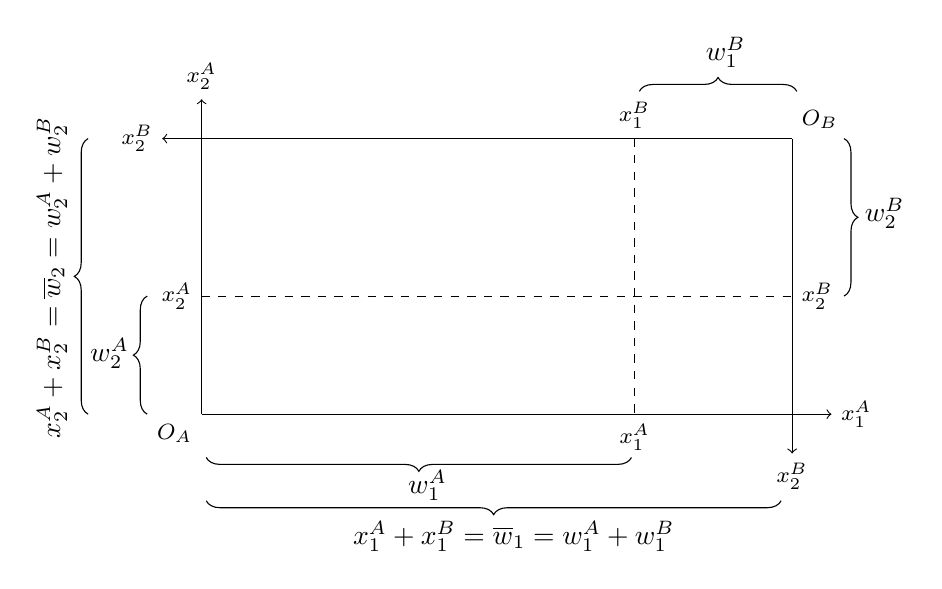
\begin{tikzpicture}[scale=1]
	% Formación de la caja
		% Consumidor A
			\draw[->] (0.5,0.5) node[align=center, below left] {\footnotesize $O_A$} -- (0.5,4.5) node[align=center, above] {\footnotesize $x_{2}^{A}$};
			\draw[->] (0.5,0.5) -- (8.5,0.5) node[align=center, right] {\footnotesize $x_{1}^{A}$};
	
		%Consumidor B
			\draw[->] (8,4) node[align=center, above right] {\footnotesize $O_B$} -- (0,4) node[align=center, left] {\footnotesize $x_{2}^{B}$};
			\draw[->] (8,4) -- (8,0) node[align=center, below] {\footnotesize $x_{2}^{B}$};
	
	% Intersección de una dotación
		\draw[dashed] (6,4) node[above] {\footnotesize $x_{1}^{B}$} -- (6,0.5) node[below] {\footnotesize $x_{1}^{A}$};
		\draw[dashed] (0.5,2) node[left] {\footnotesize $x_{2}^{A}$} -- (8,2)node[right] {\footnotesize $x_{2}^{B}$};
	
	% Llaves
		\draw [decorate,decoration={brace,amplitude=5pt},xshift=-4pt,yshift=0pt] (6.1,-0.05) -- (0.7,-0.05);
		\node [right] at (3,-0.4) {$w_{1}^{A}$};
	
		\draw [decorate,decoration={brace,amplitude=5pt},xshift=-4pt,yshift=0pt] (6.2,4.6) --(8.2,4.6);
		\node [right] at (6.78,5.1) {$w_{1}^{B}$};
		
		\draw [decorate,decoration={brace,amplitude=5pt},xshift=-4pt,yshift=0pt] (-0.05,0.5) --(-0.05,2);
		\node [left] at (-0.3,1.27) {$w_{2}^{A}$};
		
		\draw [decorate,decoration={brace,amplitude=5pt},xshift=-4pt,yshift=0pt] (8.8,4) --(8.8,2);
		\node [right] at (8.8,3.05) {$w_{2}^{B}$};
		
		\draw [decorate,decoration={brace,amplitude=5pt},xshift=-4pt,yshift=0pt] (8,-0.6) -- (0.7,-0.6);
		\node [right] at (2.3,-1.05) {$x_{1}^{A}+x_{1}^{B}=\overline{w}_1=w_{1}^{A}+w_{1}^{B}$};
		
		\draw [decorate,decoration={brace,amplitude=5pt},xshift=-4pt,yshift=0pt] (-0.8,0.5) --(-0.8,4);
		\node [left,rotate=90] at (-1.4,4.4) {$x_{2}^{A}+x_{2}^{B}=\overline{w}_2=w_{2}^{A}+w_{2}^{B}$};
\end{tikzpicture}